\documentclass[sigconf]{acmart}
% % Packages
\usepackage{soul}
% \usepackage{cite}
% \usepackage{balance}
% \usepackage{listings}
% \usepackage{amsmath,amssymb,amsfonts}
% \usepackage{algorithmic}
% \usepackage{graphicx}
% \usepackage{textcomp}
% \usepackage{xcolor}
% \usepackage{booktabs}
% \usepackage{enumitem}
% \usepackage{hyperref}
% \usepackage{totpages}
% \usepackage{subcaption}

%% \BibTeX command to typeset BibTeX logo in the docs
\AtBeginDocument{%
  \providecommand\BibTeX{{%
    \normalfont B\kern-0.5em{\scshape i\kern-0.25em b}\kern-0.8em\TeX}}}

\begin{document}

% Specify path to images
\graphicspath{ {./img/} }


%%
%% The "title" command has an optional parameter,
%% allowing the author to define a "short title" to be used in page headers.
\title[Contrast Subgraphs of Brain Networks]{Improvements and Discussion of "Explainable Classification of Brain Networks via Contrast Subgraphs"}

\author{Tengkai Yu}
\email{FIXTHIS@uvic.ca}
\affiliation{%
  \institution{University of Victoria}
  \department{Computer Science}
  \streetaddress{PO Box 1700 STN CSC}
  \city{Victoria}
  \state{British Columbia}
  \country{Canada}
  \postcode{V8W 2Y2}
}

\author{Keanelek Enns}
\email{keanelekenns@uvic.ca}
\affiliation{%
  \institution{University of Victoria}
  \department{Computer Science}
  \streetaddress{PO Box 1700 STN CSC}
  \city{Victoria}
  \state{British Columbia}
  \country{Canada}
  \postcode{V8W 2Y2}
}

%%
%% By default, the full list of authors will be used in the page
%% headers. Often, this list is too long, and will overlap
%% other information printed in the page headers. This command allows
%% the author to define a more concise list
%% of authors' names for this purpose.
\renewcommand{\shortauthors}{T. Yu and K. Enns}

%%
%% The abstract is a short summary of the work to be presented in the
%% article.
\begin{abstract}
\hl{TODO}
\end{abstract}

%%
%% The code below is generated by the tool at http://dl.acm.org/ccs.cfm.
%%
\begin{CCSXML}
<ccs2012>
   <concept>
       <concept_id>10002950.10003624.10003633.10010917</concept_id>
       <concept_desc>Mathematics of computing~Graph algorithms</concept_desc>
       <concept_significance>500</concept_significance>
       </concept>
   <concept>
       <concept_id>10010405.10010444.10010446</concept_id>
       <concept_desc>Applied computing~Consumer health</concept_desc>
       <concept_significance>300</concept_significance>
       </concept>
 </ccs2012>
\end{CCSXML}

\ccsdesc[500]{Mathematics of computing~Graph algorithms}
\ccsdesc[300]{Applied computing~Consumer health}

%%
%% Keywords. The author(s) should pick words that accurately describe
%% the work being presented. Separate the keywords with commas.
\keywords{graph analytics, graph algorithms, brain networks, densest subgraph}

\settopmatter{printfolios=true} % for page numbering

%% This command processes the author and affiliation and title
%% information and builds the first part of the formatted document.
\maketitle

\section{Introduction} \label{intro}

The question we are asking is, "Can we translate a brain network into a vector/embedding in such a way that the embedding is intuitive \emph{and} adequately separates different brain networks according to their classes?"
If we could do this, we would have an explainable classification method for brain networks.

Lanciano \emph{et al.} proposed a method that used contrast subgraphs to create two dimensional representations of brain networks \cite{lanciano2020}.
A contrast subgraph is simply a subgraph, or set of nodes, that is dense (has high edge weight) in one group of networks and sparse in another, assuming that all analyzed graphs share a common vertex set.

\section{Related Work} \label{related-work}

\hl{Are you supposed to mention the paper you are replicating in the related works? Also, to what extent should we mention the papers that Lanciano built off of?}

\hl{Talk about trend towards explainability in AI (xAI). A possible reference is https://doi.org/10.1016/j.inffus.2021.01.008}

Dai and Wang worked on creating explanations that are built into a GNN \cite{dai2021} rather than trying to find an explanation after the GNN had made its classification.
They found their method to be less biased and more computationally efficient when compared to using a post-hoc explainer such as GNN explainer.

Wang \emph{et al.} recently proposed a method, named DHC-E, for embedding graphs in a generalizable way that does not require any hyperparameters \cite{wang2021}. The embedding has a moderate number of dimensions depending on the graph set analyzed and is based on the h-index values of each node in the graph. They used principal component analysis to present the graph embeddings in two dimensions.

\hl{Look into https://doi.org/10.1142/S0129183118400077,

https://dl.acm.org/doi/abs/10.1145/3219819.3219980}

\section{Problem Statement} \label{problem-statement}

This is a special case of graph classification where all considered graphs possess the same set of vertices (i.e. regions of the brain which are, naturally, common to all brains).

\section{Experiments} \label{experiments}

\begin{figure}
    \centering
    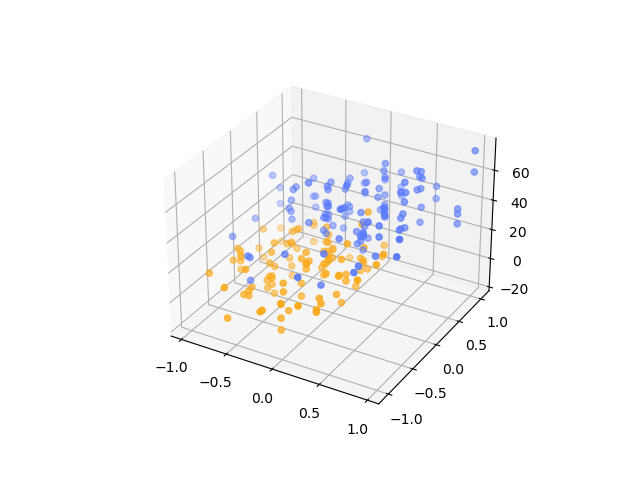
\includegraphics[width=\columnwidth, keepaspectratio=true]{test.png}
    \caption{\hl{This is just a test image, we need to create proper images with proper labels}}
    \label{fig:my_label}
\end{figure}

\section{Limitations} \label{limitations}

This study was limited primarily by the data set used.
In many machine learning applications, a large volume of data is needed to adequately train and test new models.
With a small data set, it is difficult to know how generalizable any of the discussed methods are to new brain networks that we wish to classify.
Additionally, the way the data set was created and the individuals that were studied have a large impact on the validity of the methods developed with respect to classifying brain networks with ASD.
The limitations in data set quantity and size are likely due to the costly nature of developing such brain networks as the ones analyzed in this study [\hl{TODO: back that claim up and perhaps talk about the data preparation like Lanciano did}].

Furthermore, Autism Spectrum Disorder is a very complex disorder with unclear definitions, and it may manifest in various different ways [\hl{perhaps this belongs in the intro when describing why the problem is hard?}].
Above all this, the brain is a highly complex organ that is not fully understood.
The brains of individuals are unique and develop in complex manners.
There may be a plethora of confounding factors that have an effect on the classification of such networks with respect to identifying ASD in individuals.

\section{Discussion} \label{discussion}

Lanciano \emph{et al.} showed that the degrees of each node in the studied brain networks did not vary significantly between the two classes \cite{lanciano2020},
yet the contrast subgraphs are defined as a set of nodes, and every edge induced by these nodes is used for classification.
Instead, we should look solely at edges that are important for distinguishing between the classes.

The discriminative edge method considers the most important edges in each class (defined as having the most positive and most negative weights in the difference network) when creating an embedding.
Additionally, it considers the brain network as a whole in its third dimension, which likely captures more interesting information with respect to complex connections in the brain.
However, it does not specifically identify higher order structures in the brain networks that may be leading to the DNN's success.

\section{Conclusion} \label{conclusion}

Future work should attempt to identify higher order structures (such as triangles, k-clusters, or graphlets of varying size and shapes) as a means of embedding.
This could be done by identifying prominent structures in each summary graph (perhaps after thresholding the edge weights), eliminating structures common to both, and counting the number of overlapping structures that a new brain network has in common with each class.
The challenge associated with this technique comes with the computational complexity of enumerating such high order structures.

As discussed in section \ref{limitations}, this study should be replicated on additional data sets to further test its validity.

\bibliographystyle{ACM-Reference-Format}
\bibliography{refs.bib}

\appendix
\section*{APPENDICES}
\section{Artifacts} \label{artifacts}

Project Repository:

\url{https://github.com/keanelekenns/contrast-subgraph}

\end{document}
\endinput